\documentclass{plt}
\usetikzlibrary{trees}

\title{Logic Programming: The Prolog Language}
\author{Stephen A. Edwards}
\institute{Columbia University}
\date{Fall 2018}
\titlegraphic{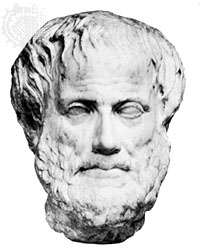
\includegraphics[width=0.25\textwidth]{aristotle.jpg}}

%\newcommand{\hlt}[1]{\textcolor{red}{#1}}
\newcommand{\lab}[3]{\tikz{\useasboundingbox (0,0);
    \node [draw=black, anchor=west,fill=black!10,rectangle callout,
      callout absolute pointer={(1pt,3pt)}]
  at (#1,#2) {\rmfamily{\textcolor{black}{#3}}}; 
}}

% Work around a tikz bug
\makeatletter
\def\pgf@test{}
\makeatother

\begin{document}

\maketitle

\begin{frame}[fragile]{Logic}

\vspace{4pt}

\hbox to \textwidth{\hfil
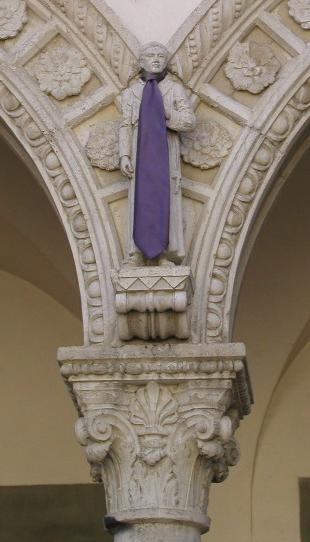
\includegraphics[height=0.4\textwidth]{caltech-tie-statue.jpg}
\hspace{3pt}
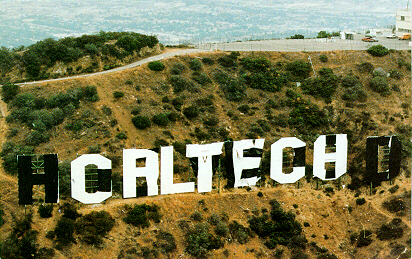
\includegraphics[height=0.4\textwidth]{caltech-hollywood-sign.jpg}
\hfil
}

\begin{center}
All Caltech graduates are nerds.

Stephen is a Caltech graduate.

Is Stephen a nerd?
\end{center}

\pause

% [user].
% |: nerd(X) :- techer(X).
% |: techer(stephen).
% CTRL-D
% yes
% ?- techer(stephen).

% Alternately, to read ``caltech.pl,''
% ?- [caltech].

\begin{columns}
  \begin{column}{0.5\textwidth}
\begin{prolog}
nerd(X) :- techer(X).

techer(stephen).
\end{prolog}
  \end{column}
  \begin{column}{0.3\textwidth}
\begin{interactive}
?- \type{nerd(stephen).}
yes
\end{interactive}
  \end{column}
\end{columns}

\end{frame}

\if 0

\hlt{caltech.pl}:
\begin{verbatim}
nerd(X) :- techer(X).
techer(stephen).
\end{verbatim}

Invoke the Prolog interpreter:

\begin{verbatim}
?- [caltech]. /* consult caltech.pl */
yes
?- nerd(stephen).
yes
\end{verbatim}

\fi

\begin{frame}[fragile]{More Logic}

\begin{prolog}
witch(X)  :- burns(X), female(X).
burns(X)  :- wooden(X).
wooden(X) :- floats(X).
floats(X) :- sameweight(duck, X).

female(girl).          /* By observation */
sameweight(duck,girl). /* By experiment */
\end{prolog}

\begin{interactive}
? \type{witch(girl).}
yes
\end{interactive}

\hfill
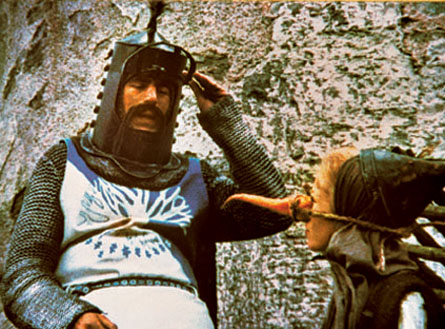
\includegraphics[width=0.4\textwidth]{monty-python-holy-grail-witch.jpg}

\end{frame}

\begin{frame}[fragile]{Still More Logic}

``My Enemy's Enemy is My Friend.''

\footnotesize

\begin{minipage}{0.5\textwidth}
\begin{prolog}
friend(X,Z) :-
   enemy(X,Y), enemy(Y,Z).

enemy(stephen, ryan).
enemy(ryan, jordan).
enemy(jordan, jacob).
\end{prolog}
\end{minipage}
\begin{minipage}{0.45\textwidth}
\begin{interactive}
?- \type{friend(stephen,jordan).}
yes
?- \type{friend(stephen,X).}
X = jordan
?- \type{friend(X, Y).}
X = stephen Y = jordan
X = ryan Y = jacob
\end{interactive}
\end{minipage}

\end{frame}

\begin{frame}
  \frametitle{The Basic Idea of Prolog}

\begin{itemize}

\item AI programs often involve searching for the solution to a problem.

\item Why not provide this search capability as the underlying idea of
the language?

\item Result: Prolog

\end{itemize}

\end{frame}

\begin{frame}{Prolog}

Mostly declarative.

Program looks like a declaration of facts plus rules for deducing
things.

``Running'' the program involves answering questions that refer to the
facts \hlt{or can be deduced from them}.

More formally, you provide the axioms, and Prolog tries to prove theorems.

\end{frame}

\begin{frame}[fragile]{Prolog Execution}

\begin{tabular}{@{}cc@{\hspace{-1pc}}c}
&& \vbox{
\hbox{\hlt{Facts}\strut}
\hbox{\begin{prolog}
nerd(X) :- techer(X).
techer(stephen).
\end{prolog}
}} \\
&& $\downarrow$ \\
\vbox{
\hbox{\hlt{Query}\strut}
\hbox{
\begin{minipage}{0.3\textwidth}
\begin{interactive}
?- \type{nerd(stephen).}
\end{interactive}
\end{minipage}
}} & $\rightarrow$ &
\hlt{Search} (Execution) \\
&& $\downarrow$ \\
&& \vbox{
\hbox{\hlt{Result}\strut}
\hbox{
\begin{minipage}{3pc}
\begin{interactive}
yes
\end{interactive}
\end{minipage}
}}
\end{tabular}

\end{frame}

\begin{frame}[fragile]
  \frametitle{Simple Searching}

Starts with the query:

\begin{minipage}{0.3\textwidth}
\begin{interactive}
?- \type{nerd(stephen).}
\end{interactive}
\end{minipage}

\emph{Can we convince ourselves that \texttt{nerd(stephen)} is true
given the facts we have?}

\begin{prolog}
techer(stephen).
nerd(X) :- techer(X).
\end{prolog}

First says \texttt{techer(stephen)} is true.  Not helpful.

Second says that we can conclude \texttt{nerd(X)} is true if we can
conclude \texttt{techer(X)} is true.  More promising.

\end{frame}

\begin{frame}[fragile]
  \frametitle{Simple Searching}

\begin{prolog}
techer(stephen).
nerd(X) :- techer(X).
\end{prolog}

\begin{minipage}{0.3\textwidth}
\begin{interactive}
?- nerd(stephen).
\end{interactive}
\end{minipage}

\emph{Unifying} \texttt{nerd(stephen)} with the head of the second
rule, \texttt{nerd(X)}, we conclude that \texttt{X = stephen}.

We're not done: for the rule to be true, we must find that all its
conditions are true.  \texttt{X = stephen}, so we want
\texttt{techer(stephen)} to hold.

This is exactly the first clause in the database; we're satisfied.
The query is simply true.

\end{frame}

\begin{frame}[fragile]
  \frametitle{More Clever Searching}

\begin{prolog}
techer(stephen).
techer(todd).
nerd(X) :- techer(X).
\end{prolog}

\begin{minipage}{0.3\textwidth}
\begin{interactive}
?- \type{nerd(X).}
\end{interactive}
\end{minipage}

``Tell me about everybody who's provably a nerd.''

As before, start with query.  Rule only interesting thing.

Unifying \texttt{nerd(X)} with \texttt{nerd(X)} is vacuously true, so
we need to establish \texttt{techer(X)}.

Unifying \texttt{techer(X)} with \texttt{techer(stephen)} succeeds,
setting \texttt{X = stephen}, but we're not done yet.

Unifying \texttt{techer(X)} with \texttt{techer(todd)} also succeeds,
setting \texttt{X = todd}, but we're still not done.

Unifying \texttt{techer(X)} with \texttt{nerd(X)} fails, returning no.

\end{frame}

\begin{frame}[fragile]
  \frametitle{More Clever Searching}

\begin{interactive}
$ \type{prolog}
GNU Prolog 1.3.0
By Daniel Diaz
Copyright (C) 1999-2007 Daniel Diaz
| ?- \type{[user].}
compiling user for byte code...
\type{techer(stephen).}
\type{techer(todd).}
\type{nerd(X) :- techer(X).}
\type{^D}
user compiled, 4 lines read - 400 bytes written, 14260 ms

yes
| ?- \type{nerd(X).}

X = stephen ? \type{;}

X = todd

yes

| ?-
\end{interactive}

\end{frame}

\begin{frame}[fragile]
  \frametitle{Order Matters}

\begin{interactive}
$ \type{prolog}
GNU Prolog 1.3.0
By Daniel Diaz
Copyright (C) 1999-2007 Daniel Diaz
| ?- \type{[user].}
compiling user for byte code...
\type{techer(todd).}
\type{techer(stephen).}
\type{nerd(X) :- techer(X).}
\type{^D}
user compiled, 4 lines read - 399 bytes written, 14027 ms

yes
| ?- \type{nerd(X).}

X = todd ? \type{;}\lab{2pc}{1pc}{Todd returned first}

X = stephen

yes

| ?-
\end{interactive}

\end{frame}


\newcommand{\tico}{\begin{tikzpicture}
    \draw circle (1pt);
  \end{tikzpicture}}

\newcommand{\ticx}{\begin{tikzpicture}
    \draw (0pt,2pt) -- (2pt,0pt)
    (0pt,0pt) -- (2pt,2pt);
  \end{tikzpicture}}

\newcommand{\tice}{\begin{tikzpicture}
    \path [use as bounding box] rectangle (2pt,2pt);
  \end{tikzpicture}}

\def\ttt #1 #2 #3 #4 #5 #6 #7 #8 #9{
  \begin{tikzpicture}
    \ttb #1 #2 #3 #4 #5 #6 #7 #8 #9
  \end{tikzpicture}}

\def\ttse #1 #2 #3 #4 #5 #6 #7 #8 #9{
  \begin{tikzpicture}
    \ttb #1 #2 #3 #4 #5 #6 #7 #8 #9
    \draw [red] (playfield.north west) -- (playfield.south east);
  \end{tikzpicture}}

\def\ttne #1 #2 #3 #4 #5 #6 #7 #8 #9{
  \begin{tikzpicture}
    \ttb #1 #2 #3 #4 #5 #6 #7 #8 #9
    \draw [red] (playfield.south west) -- (playfield.north east);
  \end{tikzpicture}}

\def\ttb #1 #2 #3 #4 #5 #6 #7 #8 #9{
  \matrix (playfield) [ampersand replacement=\&,%
    matrix of nodes,
    inner sep=0pt,
    nodes={inner sep=0pt,
      minimum width=4pt,
      minimum height=4pt}] {
    #1 \& #2 \& #3 \\
    #4 \& #5 \& #6 \\
    #7 \& #8 \& #9 \\    
  };
  \draw (playfield-1-2.north west) -- (playfield-3-2.south west);
  \draw (playfield-1-2.north east) -- (playfield-3-2.south east);
  \draw (playfield-2-1.north west) -- (playfield-2-3.north east);
  \draw (playfield-2-1.south west) -- (playfield-2-3.south east);
}


\begin{frame}[fragile]{Searching and Backtracking}

\catcode`X=\active\letX=\ticx
\catcode`O=\active\letO=\tico
\catcode`~=\active\let~=\tice

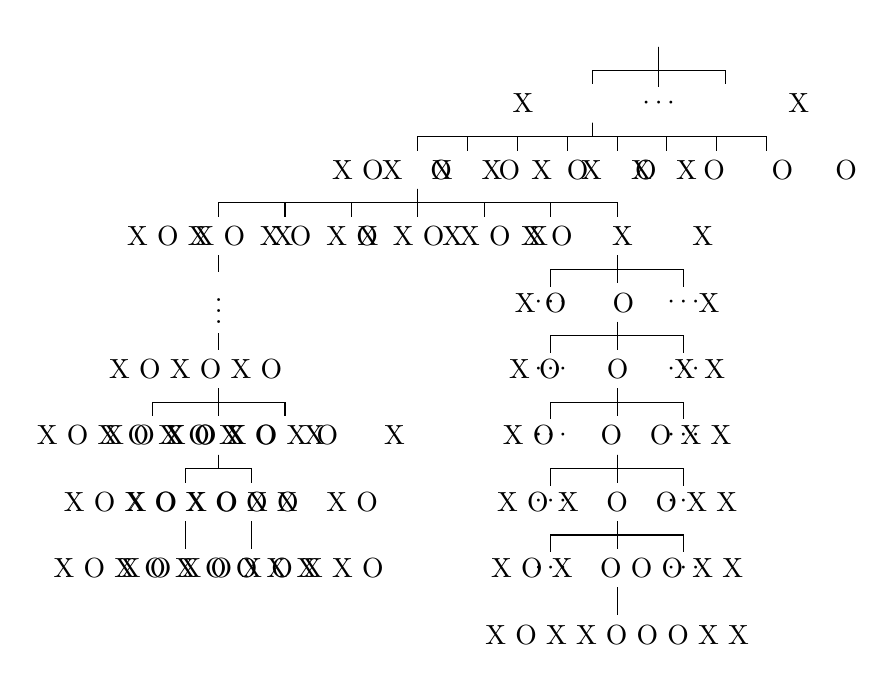
\begin{tikzpicture}
  [level distance=2pc,
    level 1/.style={sibling distance=2pc},
    level 2/.style={sibling distance=1.5pc},
    level 3/.style={sibling distance=2pc},
    edge from parent fork down
  ]
  \node {\ttt ~ ~ ~ ~ ~ ~ ~ ~ ~}
  child {node {\ttt X ~ ~ ~ ~ ~ ~ ~ ~}
    child {node {\ttt X O ~ ~ ~ ~ ~ ~ ~}
      child {node {\ttt X O X ~ ~ ~ ~ ~ ~}
        child {node {$\vdots$}
          child {node {\ttt X O X O X O ~ ~ ~}
            child {node {\ttne X O X O X O X ~ ~}}
            child {node {\ttt X O X O X O ~ X ~}
              child {node {\ttt X O X O X O O X ~}
                child {node {\ttse X O X O X O O X X}}
              }
              child {node {\ttt X O X O X O ~ X O}
                child {node {\ttne X O X O X O X X O}}
              }
            }
            child {node {\ttse X O X O X O ~ ~ X}}
          }
        }
      }
      child {node {\ttt X O ~ X ~ ~ ~ ~ ~}}
      child {node {\ttt X O ~ ~ X ~ ~ ~ ~}}
      child {node {\ttt X O ~ ~ ~ X ~ ~ ~}}
      child {node {\ttt X O ~ ~ ~ ~ X ~ ~}}
      child {node {\ttt X O ~ ~ ~ ~ ~ X ~}}
      child {node {\ttt X O ~ ~ ~ ~ ~ ~ X}
        child {node {$\cdots$}}
        child {node {\ttt X O ~ ~ O ~ ~ ~ X}
          child {node {$\cdots$}}
          child {node {\ttt X O ~ ~ O ~ ~ X X}
            child {node {$\cdots$}}
            child {node {\ttt X O ~ ~ O ~ O X X}
              child {node {$\cdots$}}
              child {node {\ttt X O X ~ O ~ O X X}
                child {node {$\cdots$}}
                child {node {\ttt X O X ~ O O O X X}
                  child {node {\ttt X O X X O O O X X}}
                }
                child {node {$\cdots$}}
              }
              child {node {$\cdots$}}
            }
            child {node {$\cdots$}}
          }
          child {node {$\cdots$}}
        }
        child {node {$\cdots$}}
      }
    }
    child {node {\ttt X ~ O ~ ~ ~ ~ ~ ~}}
    child {node {\ttt X ~ ~ O ~ ~ ~ ~ ~}}
    child {node {\ttt X ~ ~ ~ O ~ ~ ~ ~}}
    child {node {\ttt X ~ ~ ~ ~ O ~ ~ ~}}
    child {node {\ttt X ~ ~ ~ ~ ~ O ~ ~}}
    child {node {\ttt X ~ ~ ~ ~ ~ ~ O ~}}
    child {node {\ttt X ~ ~ ~ ~ ~ ~ ~ O}}
  }
  child {node {$\cdots$}}
  child {node {\ttt ~ ~ ~ ~ ~ ~ ~ ~ X}}
  ;
\end{tikzpicture}

\end{frame}

\begin{frame}[fragile]
  \frametitle{The Prolog Environment}

Database consists of \hlt{Horn clauses}. (``If a is true and b is true and ... and y is true then z is true''.)

Each clause consists of \hlt{terms}, which may be \hlt{constants},
\hlt{variables}, or \hlt{structures}.

Constants: \texttt{foo my\_Const + 1.43}

Variables: \texttt{X Y Everybody My\_var}

Structures: \begin{minipage}[t]{0.5\textwidth}
\begin{verbatim}
rainy(rochester)
teaches(edwards, cs4115)
\end{verbatim}
\end{minipage}

\end{frame}

\begin{frame}[fragile]
  \frametitle{Structures and Functors}

A structure consists of a \hlt{functor} followed by an open
parenthesis, a list of comma-separated terms, and a close parenthesis:

\vspace{3pc}

\begin{semiverbatim}
\lab{-1pc}{4.5pc}{``Functor''}bin_tree(\lab{-2pc}{2pc}{paren must follow immediately} foo, bin_tree(bar, glarch) )
\end{semiverbatim}

What's a structure?  Whatever you like.

A predicate \texttt{nerd(stephen)} \\
A relationship \texttt{teaches(edwards, cs4115)} \\
A data structure \texttt{bin(+, bin(-, 1, 3), 4)}

\end{frame}

\begin{frame}
  \frametitle{Unification}

Part of the search procedure that matches patterns.

The search attempts to match a goal with a rule in the database by
\hlt{unifying} them.

Recursive rules:

\begin{itemize}
\item A constant only unifies with itself
\item Two structures unify if they have the same functor, the same
number of arguments, and the corresponding arguments unify
\item A variable unifies with anything but forces an equivalence
\end{itemize}

\end{frame}

\begin{frame}[fragile]
  \frametitle{Unification Examples}

The \texttt{=} operator checks whether two structures unify:

\begin{interactive}
| ?- \type{a = a.}
yes                        \textrm{% Constant unifies with itself}
| ?- \type{a = b.}
no                         \textrm{% Mismatched constants}
| ?- \type{5.3 = a.}
no                         \textrm{% Mismatched constants}
| ?- \type{5.3 = X.}
X = 5.3 ? \type{;}                \textrm{% Variables unify}
yes
| ?- foo(a,X) = foo(X,b).
no                         \textrm{% X=a required, but inconsistent}
| ?- \type{foo(a,X) = foo(X,a).}
X = a                      \textrm{% X=a is consistent}
yes
| ?- \type{foo(X,b) = foo(a,Y).}                                   
X = a
Y = b                      \textrm{% X=a, then b=Y}
yes
| ?- \type{foo(X,a,X) = foo(b,a,c).} 
no                         \textrm{% X=b required, but inconsistent}
\end{interactive}


\end{frame}

\newcommand{\tab}{\hspace{2pc}}

\begin{frame}
  \frametitle{The Searching Algorithm}

\begin{tabbing}
\tab \= \tab \= \tab \= \tab \= \kill
search(goal $g$, variables $e$) \\
\>  for each clause\lab{2pc}{3pc}{in the order they appear}\ $h$ \texttt{:-} $t_1, \ldots, t_n$ in the database \\
\> \> $e = $ unify($g$, $h$, $e$)  \\
\> \> if successful, \\
\> \> \> for each term\lab{1pc}{2pc}{in the order they appear}\ $t_1, \ldots, t_n$, \\
\> \> \> \> $e = $ search($t_k$, $e$) \\
\> \> if all successful, return $e$ \\
\> return \texttt{no}
\end{tabbing}

%\rput[br](\textwidth,0){\includegraphics[width=0.4\textwidth]{map-reading.jpg}}

Note: This pseudo-code ignores one very important part of the searching process!

\end{frame}

\begin{frame}[t,fragile]
  \frametitle{Order Affects Efficiency}

\begin{columns}
  \begin{column}[t]{0.4\textwidth}

\begin{prolog}
edge(a, b). edge(b, c).
edge(c, d). edge(d, e).
edge(b, e). edge(d, f).

path(X, X).

path(X, Y) :-
    edge(X, Z), path(Z, Y).
\end{prolog}

Consider the query

\begin{interactive}
| ?- \type{path(a, a).}
\end{interactive}
  \end{column}
\begin{column}[t]{0.5\textwidth}

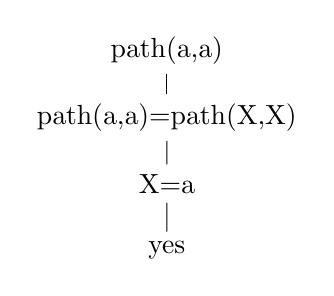
\begin{tikzpicture}
  [level distance=2pc]
  \node {path(a,a)}
  child {node {path(a,a)=path(X,X)}
    child {node {X=a}
      child {node {\hlt{yes}}}}};
\end{tikzpicture}

\end{column}
\end{columns}

Good programming practice: Put the easily-satisfied clauses first.

\end{frame}

\begin{frame}[t,fragile]
  \frametitle{Order Affects Efficiency}

\begin{columns}
  \begin{column}[t]{0.4\textwidth}

\begin{prolog}
edge(a, b). edge(b, c).
edge(c, d). edge(d, e).
edge(b, e). edge(d, f).

path(X, Y) :-
    edge(X, Z), path(Z, Y).

path(X, X).
\end{prolog}

Consider the query

\begin{interactive}
| ?- \type{path(a, a).}
\end{interactive}

Will eventually produce the right answer, but will spend much more
time doing so.

  \end{column}
\begin{column}[t]{0.5\textwidth}

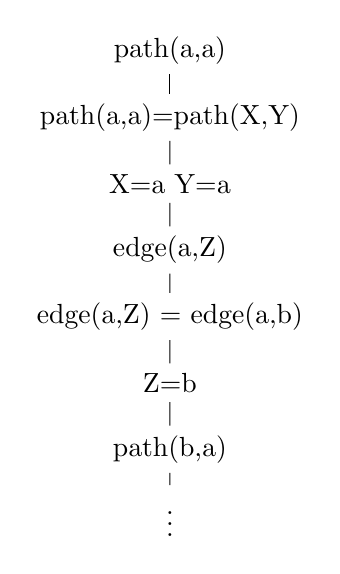
\begin{tikzpicture}
  [level distance=2pc]
  \node {path(a,a)}
  child {node {path(a,a)=path(X,Y)}
    child {node {X=a Y=a}
      child {node {edge(a,Z)}
        child {node {edge(a,Z) = edge(a,b)}
          child {node {Z=b}
            child {node {path(b,a)}
              child {node {$\vdots$}}}}}}}};
\end{tikzpicture}

\end{column}
\end{columns}

\end{frame}

\begin{frame}[t,fragile]
  \frametitle{Order Can Cause Infinite Recursion}

\begin{columns}
  \begin{column}[t]{0.4\textwidth}

\begin{prolog}
edge(a, b). edge(b, c).
edge(c, d). edge(d, e).
edge(b, e). edge(d, f).

path(X, Y) :-
    path(X, Z), edge(Z, Y).

path(X, X).
\end{prolog}

Consider the query

\begin{interactive}
| ?- \type{path(a, a).}
\end{interactive}

\centerline{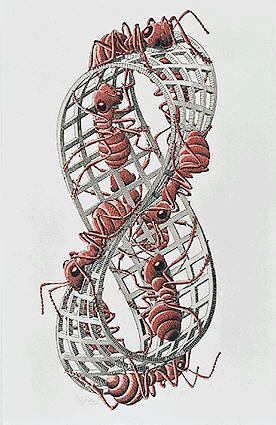
\includegraphics[width=0.4\textwidth]{escher-ants-mobeius.jpg}}

  \end{column}
\begin{column}[t]{0.5\textwidth}

\fontsize{9}{9}\selectfont

\begin{tikzpicture}
  [level distance=1.8pc,sibling distance=4pc]
  \node {path(a,a)\lab{1pc}{1pc}{Goal}}
  child {node {path(a,a)=path(X,Y)\lab{1pc}{1pc}{Unify}}
    child {node {X=a Y=a\lab{1pc}{1pc}{Implies}}
      child {node {\lab{-4pc}{1pc}{Subgoal}path(a,Z)}
        child {node {path(a,Z) = path(X,Y)}
          child {node {X=a Y=Z}
            child {node {path(a,Z)}
              child {node {path(a,Z) = path(X,Y)}
                child {node {X=a Y=Z}
                  child {node {$\vdots$}}
                }
              }
            }
            child {node {edge(Z,Z)}}
          }
        }
      }
      child {node {edge(Z,a)}}
    }
  };
\end{tikzpicture}

\end{column}
\end{columns}

\end{frame}

\begin{frame}[fragile]
  \frametitle{Bill and Ted in Prolog}

\begin{columns}
  \begin{column}{0.4\textwidth}
\href{http://www.cs.columbia.edu/~sedwards/classes/2010/w4115-fall/billnted.mp4}{
\includegraphics[width=\textwidth]{bill-and-teds-movie-poster.jpg}}
  \end{column}
  \begin{column}{0.5\textwidth}

\begin{prolog}
super_band(X) :-
   on_guitar(X, eddie_van_halen).

on_guitar(X, eddie_van_halen) :-
   triumphant_video(X).

triumphant_video(X) :-
   decent_instruments(X).

decent_instruments(X) :-
   know_how_to_play(X).

know_how_to_play(X) :-
   on_guitar(X, eddie_van_halen).
\end{prolog}

\begin{interactive}
| ?- \type{super_band(wyld_stallyns).}
\end{interactive}

\hlt{What will Bill and Ted do?}

  \end{column}
\end{columns}

{\footnotesize
\url{http://www.cs.columbia.edu/~sedwards/classes/2010/w4115-fall/billnted.mp4}}

\end{frame}

\begin{frame}[fragile]
  \frametitle{Prolog as an Imperative Language}

  \begin{columns}
    \begin{column}{0.6\textwidth}

\parskip=1pc

A declarative statement such as

\shadowstart
P if Q and R and S
\shadowend

can also be interpreted procedurally as

\shadowstart
To solve P, solve Q, then R, then S.
\shadowend

This is the problem with the last path example.

\begin{prolog}
path(X, Y) :-
   path(X, Z), edge(Z, Y).
\end{prolog}

``To solve P, solve P\ldots''
    \end{column}
    \begin{column}{0.4\textwidth}

\begin{prolog}
go :- print(hello_),
      print(world).
\end{prolog}

\begin{interactive}
| ?- \type{go.}
hello_world
yes
\end{interactive}
    \end{column}
  \end{columns}

\end{frame}

\begin{frame}[fragile]{Cuts}

  \begin{columns}
    \begin{column}{0.5\textwidth}

Ways to shape the behavior of the search:

\begin{itemize}

\item Modify clause and term order.

 Can affect efficiency, termination.

\item ``Cuts''

Explicitly forbidding further backtracking.

\end{itemize}

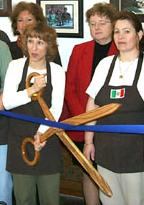
\includegraphics[width=0.5\textwidth]{big-scissors.jpg}

    \end{column}
    \begin{column}{0.5\textwidth}

When the search reaches a cut (\texttt{!}), it does no more
backtracking.

\begin{prolog}
techer(stephen) :- !.
techer(todd).
nerd(X) :- techer(X).
\end{prolog}

\begin{interactive}
| ?- \type{nerd(X).}

X = stephen

yes
\end{interactive}   

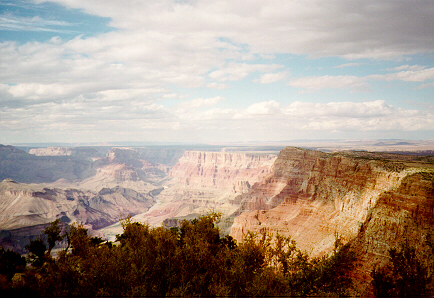
\includegraphics[width=0.6\textwidth]{grand-canyon.jpg}
    \end{column}
  \end{columns}

\end{frame}

\begin{frame}
  \frametitle{Controlling Search Order}

Prolog's ability to control search order is crude, yet often critical for both efficiency and termination.

\begin{itemize}
\item Clause order

\item Term order

\item Cuts
\end{itemize}

Often very difficult to force the search algorithm to do what you want.

\end{frame}


\begin{frame}[fragile]
  \frametitle{Elegant Solution Often Less Efficient}

Natural definition of sorting is inefficient:

\begin{prolog}
sort(L1, L2) :- permute(L1, L2), sorted(L2).
permute([], []).
permute(L, [H|T]) :-
  append(P, [H|S], L), append(P, S, W), permute(W, T).
\end{prolog}

Instead, need to make algorithm more explicit:

\begin{prolog}
qsort([], []).
qsort([A|L1, L2) :- part(A, L1, P1, S1),
  qsort(P1, P2), qsort(S1, S2), append(P2, [A|S2], L2).
part(A, [], [], []).
part(A, [H|T], [H|P], S) :- A >= H, part(A, T, P S).
part(A, [H|T], P, [H|S]) :- A < H, part(A, T, P S).
\end{prolog}

\end{frame}

\begin{frame}
  \frametitle{Prolog's Failings}

Interesting experiment, and probably perfectly-suited if your problem
happens to require an AI-style search.

Problem is that if your peg is round, Prolog's square hole is
difficult to shape.

No known algorithm is sufficiently clever to do smart searches in all
cases.

Devising clever search algorithms is hardly automated: people get
PhDs for it.

\end{frame}

\end{document}

% Local Variables:
% mode: latex
% compile-command: "make prolog.pdf"
% End:


